% ================================ L'ALGORITMO ========================================

\chapter{L'Algoritmo} %TODO: Rinominare in "Una panoramica sull'Algoritmo" o in realtà quello è per una sezione?

%TODO: Le varie sezioni: sub bytes, Shift Rows, mix columns, Add Round Key
%TODO: aggiungere immagini

%TODO: perché l'ultimo round è differente?

%TODO: 1. KeyExpansion (Rijndael Key Scheduler/AES Key Scheduler)
%TODO: 1. AddRoundKey (con lo XOR)

%TODO: 1. SubBytes (S-Box)
%TODO: 2. ShiftRows (1a riga niente, 2a riga = shift a sinistra di 1, 3a riga = shift di 2, 4a riga = shift di 3) (lo shift è come una ROL in x86)
%TODO: 3. MixColumns (Rijndael Key Scheduler/AES Key Scheduler)
%TODO: 4. AddRoundKey (con lo XOR)

%TODO: ShiftRows e MixColumns per la "Confusione e Diffusione" (teoria di Shannon).

%TODO: 10 rounds (fasi/cicli) per chiavi di 128-bit
%TODO: 12 rounds (fasi/cicli) per chiavi di 192-bit
%TODO: 14 rounds (fasi/cicli) per chiavi di 256-bit

% ======================================================================================

% ---------------------------- SECTION: INTRODUZIONE ----------------------------------

%\newpage

\section{Introduzione}

\textsf{\small In questo capitolo, tratteremo il funzionamento dell'algoritmo di AES con una panoramica dall'alto, per poi affrontare nel prossimo capitolo, più in dettaglio, la sua matematica.}

% ----------------- SECTION: I TRE CONCETTI DIETRO LA CRITTOGRAFI ----------------------

%\newpage

\section{I tre concetti dietro la Crittografia} %TODO: Le tre idee/concetti/principi dietro la/alla Crittografia

\textsf{\small Alla base della crittografia, ci sono due importanti proprietà dei cifrari a chiave simmetrica, elaborati dal padre della teoria dell'informazione, Claude Elwood Shannon, ovvero: \emph{diffusione} e \emph{confusione}.} \\

\begin{comment}
\begin{figure}[H]
	\centering
	\includegraphics[width=1\textwidth, height=1\textheight, keepaspectratio]{./images/theory_of_information/confusion_and_diffusion.png}
	\caption{Confusion and Diffusion}
	\label{fig:confusion_and_diffusion2}
\end{figure}
\end{comment}

%TODO: itemize?

\textsf{\small Il principio della \emph{confusione} vela la connessione tra il messaggio originale e il testo cifrato.} %TODO: messaggio/testo; [per esempio cifrario di cesare (con annessa immagine volendo)]

\textsf{\small La proprietà di \emph{diffusione}, invece, riguarda lo scombussolamento della posizione dei caratteri del messaggio.} %TODO: [un semplice esempio potrebbe essere la trasposizione delle colonne in una matrice oppure non lo scrivo.]

\textsf{\small Un altro importante concetto è quello della \emph{segretezza della chiave}, ovvero che l'algoritmo alla base del cifrario è conosciuto, è pubblico, ma la sola conoscenza di questo non è sufficiente per poter conseguire l'accesso alle informazioni, perché per poter attingerle sarà necessario conoscere la chiave segreta.} %TODO: nella/della chiave; attingere/ottenere; attingerle/acquisire/raggiungere; concetto/astrazione

\begin{figure}[H]
	\centering
	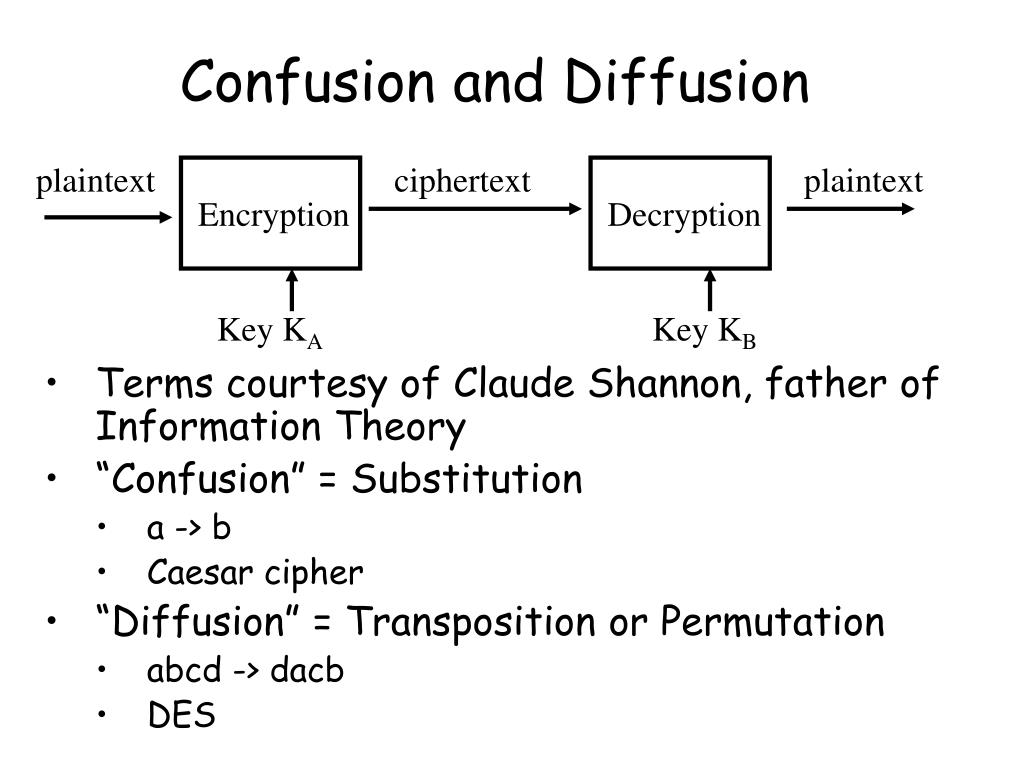
\includegraphics[width=1\textwidth, height=1\textheight, keepaspectratio]{./images/theory_of_information/confusion-and-diffusion.png}
	\caption{Confusione e Diffusione}
	\label{fig:confusion_and_diffusion}
\end{figure}

%TODO: [volendo aggiungere altro sulla teoria dell'informazione, su Shannon, sull'importanza, ecc. Magari aggiungere anche un'immagine.]

%TODO: [aggiungere una o più immagini sulla teoria di Shannon]

% ------------------- SECTION: UNA PANORAMICA SULL'ALGORITMO --------------------------

\section{Una panoramica sull'Algoritmo} %TODO: Una panoramica dell'Algoritmo/Una panoramica sull'Algoritmo (meglio una panoramica sull'algoritmo come nome!) oppure "L'Algoritmo in breve" o "Semplice Overview dell'Algoritmo".

%TODO: itemize?
%TODO: forse dovrei semplificarlo un attimo e parlarne più con calma prima di passare alle liste delle operazioni.

\textsf{\small I dati di input vengono caricati in una matrice 4x4, anche chiamata \emph{state matrix} (matrice di stato), dove ogni cella rappresenta 1 byte di informazione e su queste compiamo diverse operazioni: \emph{sub-bytes} (sostituzione dei bytes), \emph{shift rows} (spostamento delle righe), \emph{mix columns} (mescolamento delle colonne), \emph{add round key} (aggiunta della chiave del round) per un numero di volte, di rounds pari alla grandezza della chiave.} %TODO: oppure metterli in un itemize?

\begin{figure}[H]
	\centering
	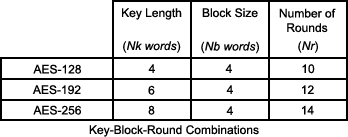
\includegraphics[width=0.8\textwidth, height=0.8\textheight, keepaspectratio]{./images/aes/key_size_and_number_of_rounds.png}
	\caption{Key Size e Numero di Rounds}
	\label{fig:aes_key_size_number_of_rounds}
\end{figure}

\textsf{\small Nel primo round svolgiamo uno XOR tra il messaggio d'input e la chiave segreta.}

\textsf{\small Lo \emph{XOR} (\emph{E\textbf{X}clusive-\textbf{OR}}) bit-a-bit è un'operazione di macsheratura dei bit, dove se i due bit di input sono diversi, allora produrrà un 1 in uscita, altrimenti se sono uguali, uno zero.} 

\begin{figure}[H]
	\centering
	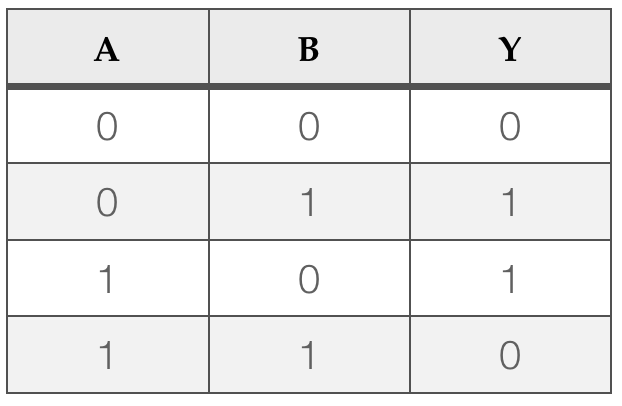
\includegraphics[width=0.6\textwidth, height=0.6\textheight, keepaspectratio]{./images/XOR/XOR-Truth-Table.png}
	\caption{Tabella della verità dello XOR}
	\label{fig:xor_truth_table}
\end{figure}

\subsection{Perché lo XOR è usato in crittografia?}

\begin{itemize}
	\item \textsf{\small Lo XOR non \emph{leaka} informazioni sull'input originale.} %TODO: magari leaka non è proprio il top come parola, non esiste nemmeno in italiano
	\item \textsf{\small Lo XOR è una \emph{involutory function} (funzione involutoria) tale che se la applichi due volte riottieni il testo originale.}
	\item \textsf{\small L'output dello XOR dipende da entrambi gli input. Non è così per le altre operazioni (AND, OR, NOT, ecc.).}
\end{itemize}

\fleuron

%TODO: magari semplificare questa parte.

\textsf{\small Per poter elaborare i rounds, l'algoritmo ha bisogno di molte chiavi, una per round, queste vengono tutte derivate dalla chiave iniziale.}

%TODO: Fare una subsection?: titolo: "Come vengono ottenute le chiavi per ogni round?" oppure no? KEY EXPANSION/KEY SCHEDULE
%TODO: Per poter eseguire/elaborare i rounds, l'algoritmo ha bisogno di molte chiavi [una per round?], queste vengono tutte derivate dalla chiave iniziale. (volendo scrivere: Questo è uno dei motivi per cui AES viene criticato, perché tutte le chiavi vengono derivate dalla chiave originale).

\textsf{\small Il procedimento per ricavarle è questo: }

\begin{enumerate}
	\item \textsf{\small Sposta la prima cella dell'ultima colonna della precedente chiave in fondo alla colonna.} %TODO: spostare
	\item \textsf{\small Ogni byte viene posto in una substitution box che lo mapperà in qualcos'altro.} %TODO: (S-box) dopo substitution box; specificare cosa quel qualcos'altro.
	\item \textsf{\small Viene effettuato uno XOR tra la colonna e una \emph{round constant} (costante di round) che è diversa per ogni round.} %TODO: approfondire come è diversa.
	\item \textsf{\small Infine viene realizzato uno XOR con la prima colonna della precedente chiave.}
	%\item \textsf{\small }
\end{enumerate}

\textsf{\small Per le altre colonne, vengono semplicemente eseguiti degli XOR con la stessa colonna della precedente chiave (eccetto per le chiavi a 256 bit che hanno un procedimento un po' più complicato).} \\ %TODO: rimuovere la parte tra parentesi? ovvero la parte procedimento un po' più complicato o approfondirla?

\begin{figure}[H] %TODO: Cambiare immagine?
	\centering
	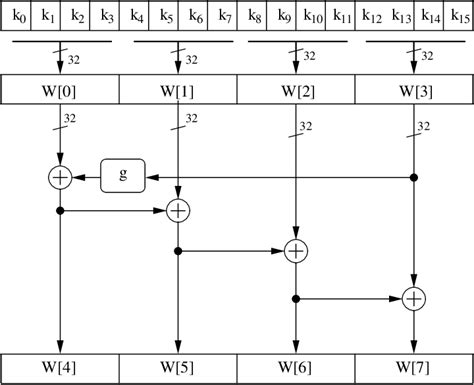
\includegraphics[width=0.8\textwidth, height=0.8\textheight, keepaspectratio]{./images/key_expansion/key_expansion.png}
	\caption{Key Expansion}
	\label{fig:key_expansion}
\end{figure}

%TODO: [mettere delle immagini a riguardo]

%TODO: Per quanto riguarda le altre colonne, vengono semplicemente eseguiti degli XOR con la stessa colonna della precedente chiave. [magari spiegare meglio] [magari mettere un'immagine a riguardo] [eccetto per le chiavi a 256 bit che sono un po' più complicate] [approfondire il perché siano più complicate]

%TODO: Dopo aver ottenuto queste chiavi vengono compiuti i vari rounds.

\textsf{\small Dopo aver ottenuto le chiavi, vengono compiuti i vari rounds.} 

\textsf{\small Per ogni round, eseguiamo questi passaggi, tranne per l'ultimo dove non effettuiamo il passaggio delle \emph{Mix Columns}, perché non aumenterebbe la sicurezza e semplicemente rallenterebbe: } %TODO: [magari approfondire il perché rallenterebbe]

\begin{itemize}
	\item[] \textsf{\small Applichiamo il principio di \emph{confusione} attraverso il passaggio \emph{Sub-bytes}.}
	\item \textsf{\small \underline{\emph{Sub-bytes}}: Ogni byte viene mappato in un diverso byte attraverso una s-box. Questo step applica la proprietà di \emph{confusione} di Shannon, perché oscura la relazione tra ogni byte.}
	\item[] \textsf{\small Applichiamo la proprietà di \emph{diffusione}:}
	\item \textsf{\small \underline{\emph{Shift Rows}}: La seconda riga della matrice viene spostata di 1 verso sinistra. La terza riga di 2 posizioni e la quarta di 3 (sempre verso sinistra).}
	\item \textsf{\small \underline{\emph{Mix Columns}}: Ogni bit delle colonne della matrice (di stato) vengono mischiate.} %TODO: Approfondire come vengono mischiate
	\item[] \textsf{\small Applichiamo la proprietà di \emph{segretezza della chiave}:}
	\item \textsf{\small \underline{\emph{Add Round Key}}: Viene applicata la chiave del prossimo round attraverso uno XOR.} %TODO: applicata, meglio trovare un altro verbo
\end{itemize}

\begin{figure}[H] %TODO: Cambiare immagine?
	\centering
	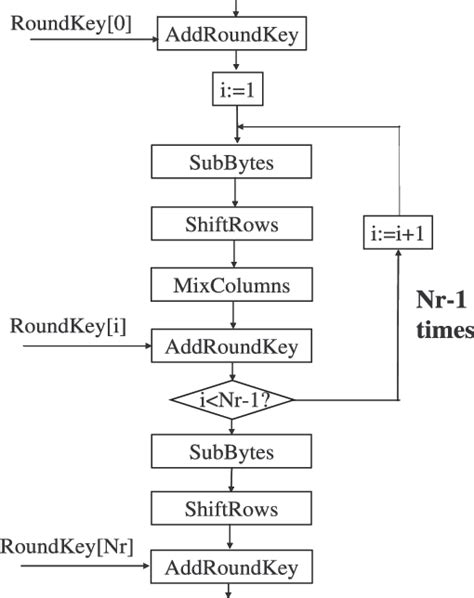
\includegraphics[width=0.5\textwidth, height=0.5\textheight, keepaspectratio]{./images/aes/flowcharts/aes_flowchart.png}
	\caption{AES Rounds Flowchart}
	\label{fig:aes_flowchart2}
\end{figure}

\textsf{\small Più rounds aggiungiamo, più sicurezza, ma questo porterebbe ad un rallentamento dell'algoritmo e quindi delle performance.}
\textsf{\small Per questo serve un compromesso tra sicurezza e prestazioni.}

\textsf{\small Quando AES era in sviluppo venne trovata una scorciatoia attraverso 6 rounds, per evitare ciò, sono stati aggiunti 4 rounds extra, come \emph{margine di sicurezza}.} %TODO: Quando AES era in sviluppo venne trovata una scorciatoia attraverso 6 rounds, [come possiamo notare ogni bit di output di un round dipende da ogni bit dei due rounds precedenti ] per evitare questo sono stati aggiunti 4 rounds extra, come \emph{margine di sicurezza}. %TODO: magari approfondire?

%TODO: [magari aggiungere qualche immagine sul procedimento]

%TODO: la subsection modalità di AES magari la sposto in un capitolo a parte? Oppure semplicemente ampio con le modalità di AES.

\subsection{Le modalità di AES} %TODO: section/subsection: "Come può essere usato AES?" o "Con quali combinazioni può essere usato AES" o "In combinazione a cosa può essere usato AES"? o "Le modalità di AES"

\textsf{\small AES non può essere utilizzato così com'è, ma necessita di essere adoperato in combinazione a una modalità. } %TODO: AES non può essere usato così com'è, ma necessita di essere utilizzato in combinazione a una modalità .
\textsf{\small Una modalità è un processo/sistema/procedimento per aumentare/incrementare/trasformare/avanzare l'efficacia di un algoritmo crittografico.  } %TODO: processo/sistema/procedimento; aumentare/incrementare/trasformare/avanzare;

\textsf{\small Di seguito, alcune delle modalità di AES: }

\begin{itemize} %TODO: approfondirli, scrivere qualcosa di ciascuno
	\item \textsf{\small \textbf{ECB} (\emph{\textbf{E}lectronic \textbf{C}ode \textbf{B}ook})}
	\item \textsf{\small \textbf{CBC} (\emph{\textbf{C}ipher \textbf{B}lock \textbf{C}haining})}
	\item \textsf{\small \textbf{CFB} (\emph{\textbf{C}ipher \textbf{F}eed\textbf{B}ack)}}
	\item \textsf{\small \textbf{OFB} (\emph{\textbf{O}utput \textbf{F}eed\textbf{B}ack)}}
	\item \textsf{\small \textbf{CTR} (\emph{\textbf{C}oun\textbf{t}e\textbf{r} mode})}
	%\item \textsf{\small }
\end{itemize} 

%TODO: magari approfondire queste modalità oppure più tardi oppure scrivere giusto un filino per ognuna e poi al massimo lo riprendo dopo.

\newpage

\begin{comment}
\begin{figure}[H] %TODO: oppure mettere un'immagine sulle modalità, oppure mettere quueta prima delle modalità %TODO: remove visto che l'ho messo nel titolo?
	\centering
	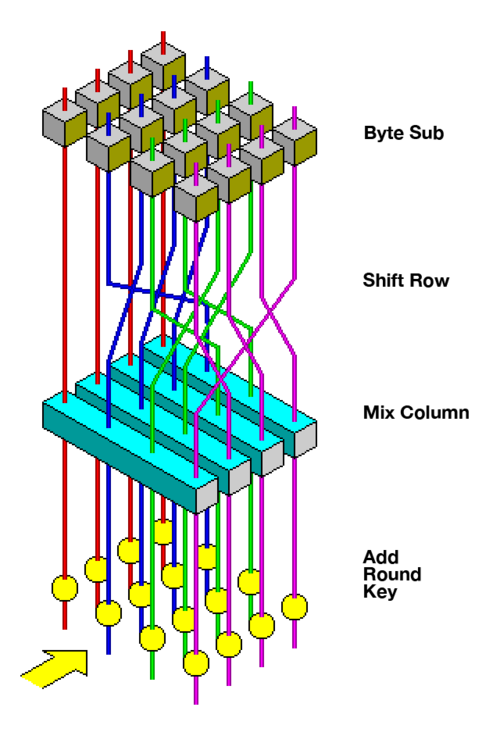
\includegraphics[width=0.6\textwidth, height=0.6\textheight, keepaspectratio]{./images/aes/500px-AES_(Rijndael)_Round_Function.png}
	\caption{AES Round Function}
	\label{fig:500px-AES_(Rijndael)_Round_Function}
\end{figure}
\end{comment}

%TODO: Approfondirli magari nella sezione dei pro e contro e dei possibili attacchi come: PA (Padding Attack), CPA (Chosen Plaintext Attack), CCA (Chosen Ci)

% -------------------------------- FINE CAPITOLO --------------------------------------